\documentclass[12pt, psamsfonts]{amsart}

%-------Packages---------
\usepackage{amssymb,amsfonts}
\usepackage{mathtools}
\usepackage{semantic}
\usepackage{fullpage}
\usepackage{tikz-cd}
\usepackage{todonotes}
\usepackage{physics}
\usepackage[all,arc]{xy}
\usepackage{enumerate}
\usepackage{enumitem}
\usepackage{mathrsfs}
\usepackage{theoremref}
\usepackage{graphicx}
\usepackage[bookmarks]{hyperref}

%--------Theorem Environments--------
%theoremstyle{plain} --- default
\newtheorem{thm}{Theorem}[section]
\newtheorem{cor}[thm]{Corollary}
\newtheorem{prop}[thm]{Proposition}
\newtheorem{lem}[thm]{Lemma}
\newtheorem{conj}[thm]{Conjecture}
\newtheorem{quest}[thm]{Question}

\theoremstyle{definition}
\newtheorem{defn}[thm]{Definition}
\newtheorem{defns}[thm]{Definitions}
\newtheorem{con}[thm]{Construction}
\newtheorem{exmp}[thm]{Example}
\newtheorem{exmps}[thm]{Examples}
\newtheorem{notn}[thm]{Notation}
\newtheorem{notns}[thm]{Notations}
\newtheorem{addm}[thm]{Addendum}
\newtheorem*{exer}{Exercise}

\theoremstyle{remark}
\newtheorem{rem}[thm]{Remark}
\newtheorem{rems}[thm]{Remarks}
\newtheorem{warn}[thm]{Warning}
\newtheorem{sch}[thm]{Scholium}

\DeclareMathOperator{\Hom}{Hom}
\DeclareMathOperator{\Id}{Id}
\DeclareMathOperator{\End}{End}
\DeclareMathOperator{\ord}{ord}
\DeclareMathOperator{\Aut}{Aut}
\DeclareMathOperator{\Gal}{Gal}
\DeclareMathOperator{\Int}{Int}
\DeclareMathOperator{\RP}{\mathbb{R}\mathbf{P}}

\makeatletter
\let\c@equation\c@thm
\makeatother
\numberwithin{equation}{section}

\bibliographystyle{plain}

\begin{document}

\title{Math 611 Final}
\author{Hidenori Shinohara}
\maketitle


\begin{exer}{(Problem 1(a))}
  \begin{figure}[!htb]
    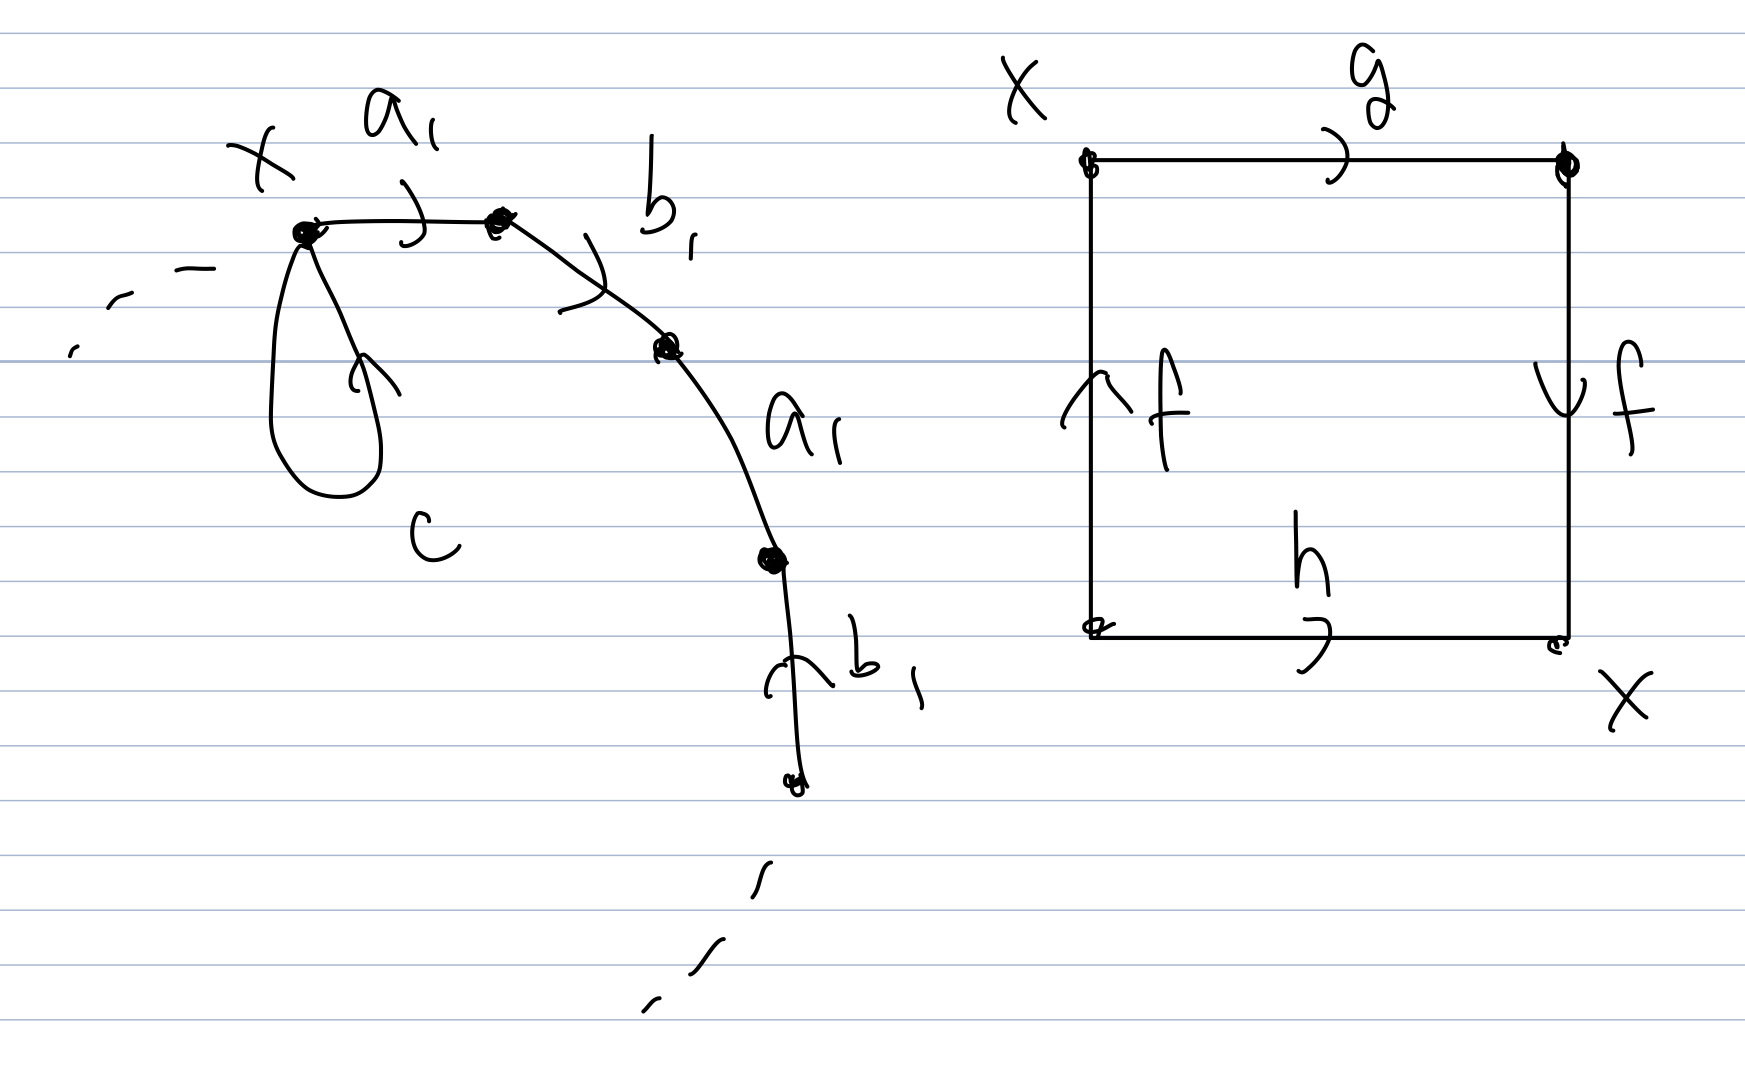
\includegraphics[width=.7\linewidth]{problem1_a.jpeg}
    \caption{Problem 1(a)}
    \label{fig:problem1a}
  \end{figure}
  We will use the 1-skeletons in Figure \ref{fig:problem1a} to calculate the fundamental group of $S$.
  The fundamental group of the left side with a 2-cell attached is $\ev{a_1, b_1, \cdots, a_g, b_g, c \mid [a_1, b_1] \cdots [a_g, b_g]c}$, and the right side is $\ev{gf, f^{-1}h \mid gfh^{-1}f}$.
  By Van Kampen, the fundamental group of $S$ is 
  \begin{align*}
    \ev{ a_1, b_1, \cdots, a_g, b_g, c, gf, f^{-1}h \mid [a_1, b_1] \cdots [a_g, b_g]c, gfh^{-1}f, c(gh)^{-1}}
  \end{align*}
  where $c(gh)^{-1}$ corresponds to $i_{\alpha\beta}(c)i_{\beta\alpha}(c)^{-1}$ because we identify $c$ with $gh$.
  Let $\alpha = gf, \beta = f^{-1}h$.
  Then
  \begin{align*}
    &\ev{ a_1, b_1, \cdots, a_g, b_g, c, gf, f^{-1}h \mid [a_1, b_1] \cdots [a_g, b_g]c, gfh^{-1}f, c(gh)^{-1}} \\
    &\cong \ev{ a_1, b_1, \cdots, a_g, b_g, c, \alpha, \beta \mid [a_1, b_1] \cdots [a_g, b_g]c, \alpha\beta^{-1}, c(\alpha\beta)^{-1}} \\
    &\cong \ev{ a_1, b_1, \cdots, a_g, b_g, c, \alpha \mid [a_1, b_1] \cdots [a_g, b_g]c, c\alpha^{-2}} \\
    &\cong \ev{ a_1, b_1, \cdots, a_g, b_g, \alpha \mid [a_1, b_1] \cdots [a_g, b_g]\alpha^2}.
  \end{align*}
\end{exer}

\begin{exer}{(Problem 1(b))}
  \begin{figure}[!htb]
    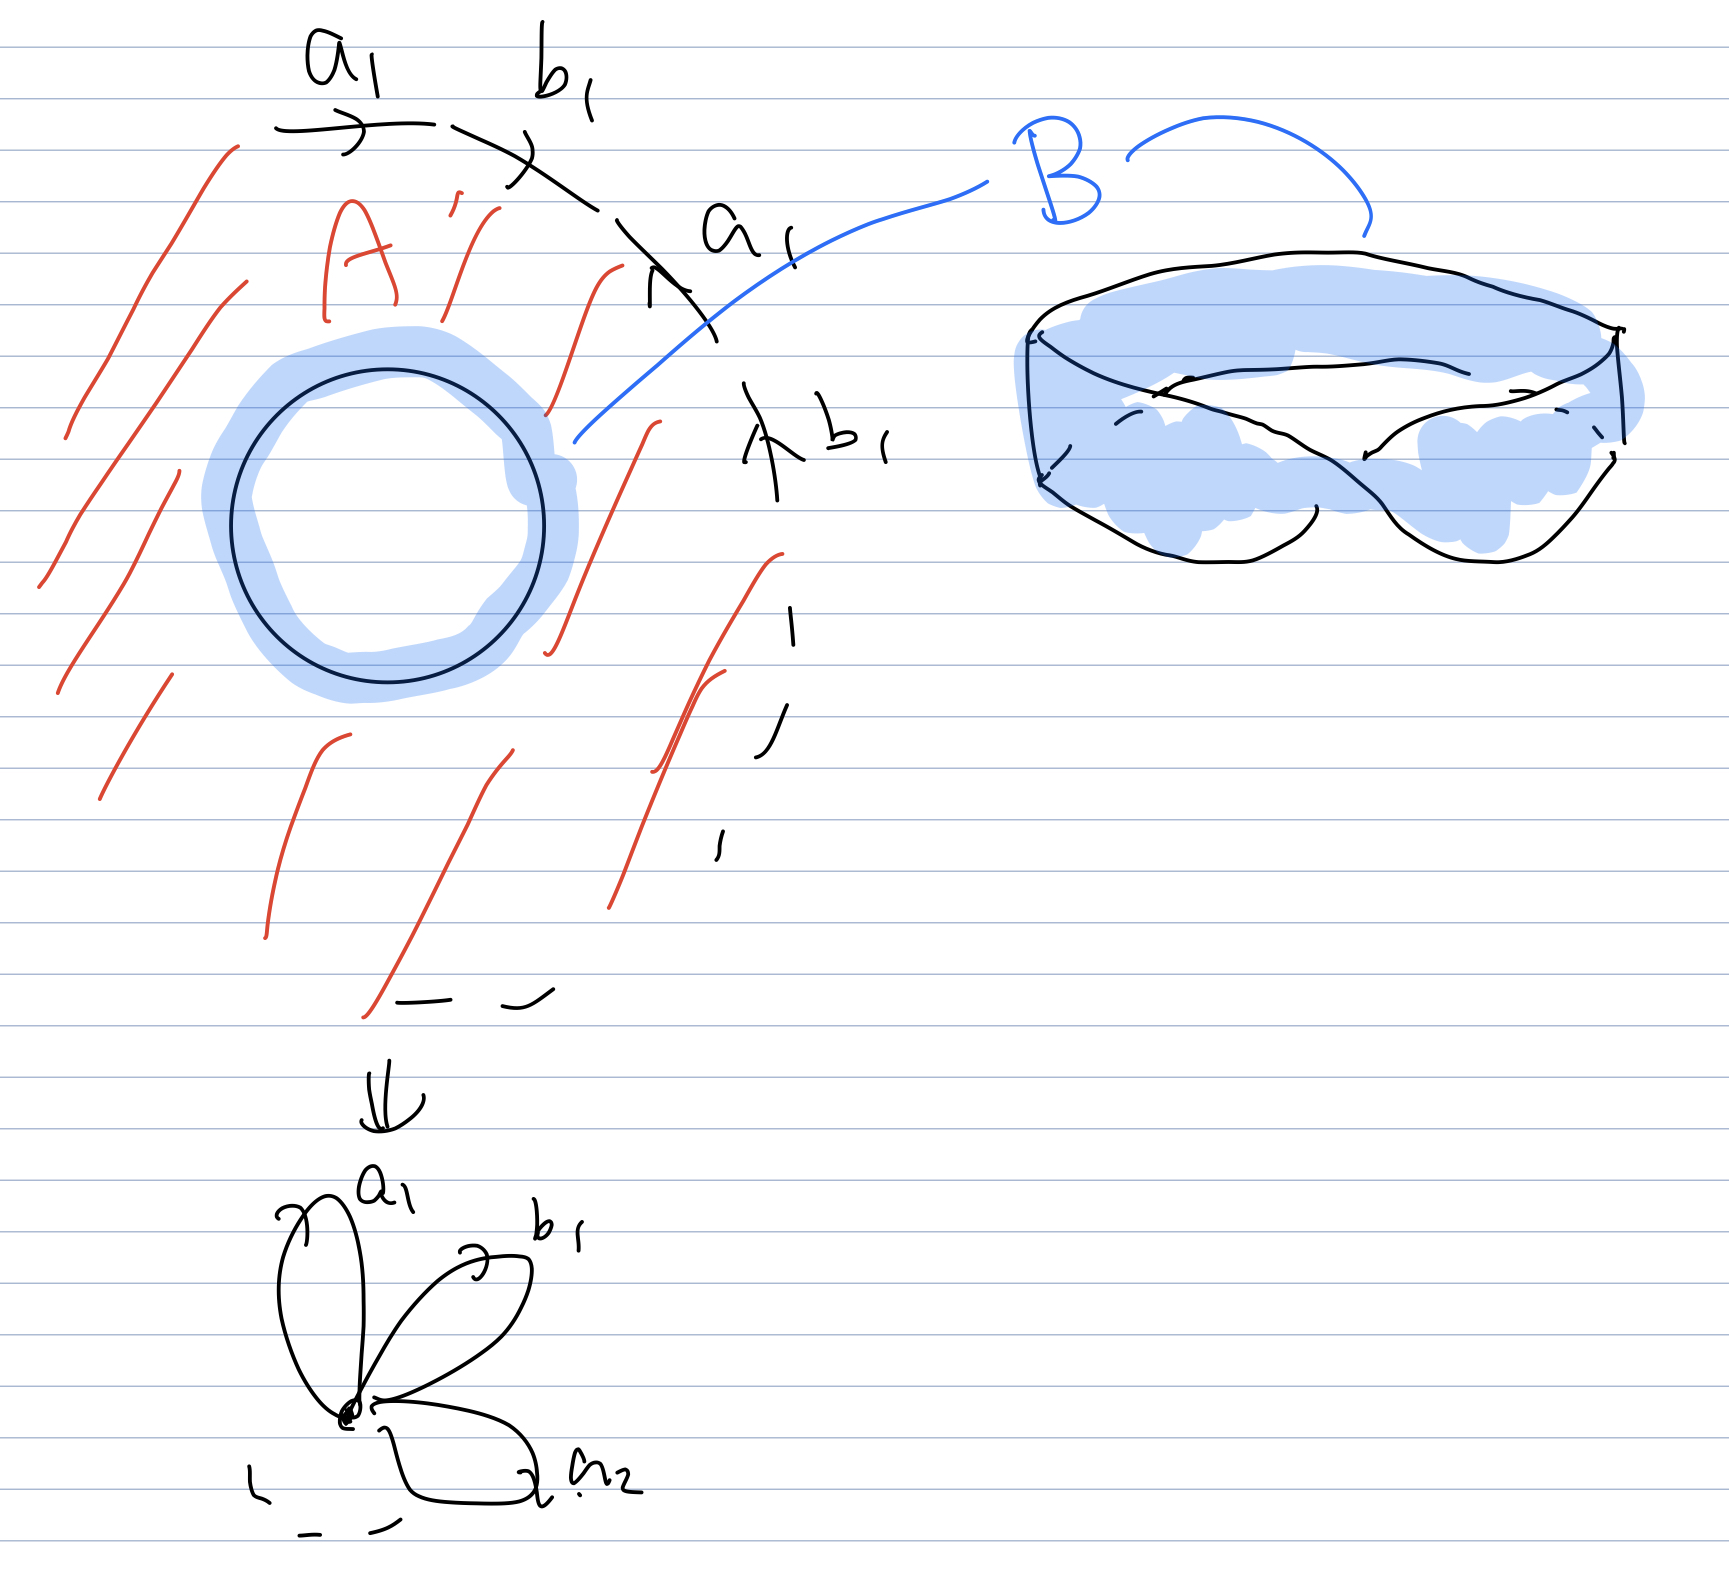
\includegraphics[width=.7\linewidth]{Mg.jpeg}
    \caption{$M_g$ with the Mobius band}
    \label{fig:mg}
  \end{figure}
  Let $A = \Sigma_g \setminus D^2$ and $B$ be a Mobius strip $M$ with some neighborhood from $\Sigma_g$ such that $\Int(A) \cup \Int(B) = S$ as in Figure \ref{fig:mg}.
  Then $A$ is homotopy equivalent to the wedge sum of $2g$ $S^1$'s.
  Moreover, $B$ is homotopy equivalent to $S^1$ and so is $A \cap B$.
  We will consider the Mayer-Vietoris sequence formed by $A, B \subset X$.

  We will start with the sequence $H_n(A) \oplus H_n(B) \rightarrow H_n(A \cup B) \rightarrow H_{n - 1}(A \cap B)$ where $n - 1 \geq 2$.
  Then $H_n(A) = H_n(B) = H_{n - 1}(A \cap B) = 0$ for $n \geq 3$.
  By exactness, $H_n(A \cup B) = 0$ when $n \geq 3$.

  We will consider the following exact sequence:

  \begin{align*}
    &\tilde{H}_2(A \cap B) \rightarrow \tilde{H}_2(A) \oplus \tilde{H}_2(B) \rightarrow \tilde{H}_2(X) \xrightarrow{\alpha} \\
    &\tilde{H}_1(A \cap B) \xrightarrow{\beta} \tilde{H}_1(A) \oplus \tilde{H}_1(B) \xrightarrow{\gamma} \tilde{H}_1(X) \rightarrow \\
    &\tilde{H}_0(A \cap B).
  \end{align*}

  Then $\tilde{H}_2(A) = \tilde{H}_2(B) = \tilde{H}_0(A \cap B) = 0$.
  Thus the above sequence can be simplified to 
  \begin{align*}
    0 \rightarrow \tilde{H}_2(X) \xrightarrow{\alpha} &\tilde{H}_1(A \cap B) \xrightarrow{\beta} \tilde{H}_1(A) \oplus \tilde{H}_1(B) \xrightarrow{\gamma} \tilde{H}_1(X) \rightarrow 0.
  \end{align*}
  Since the sequence is exact, $\alpha$ must be injective and $\gamma$ must be surjective.
  We will examine $\beta$ to calculate the homology groups.
  Since $A \cap B$ is homotopy equivalent to $S^1$, $\tilde{H}_1(A \cap B) = \mathbb{Z}$.
  By Corollary 2.25, $\tilde{H}_1(A) = \mathbb{Z}^{2g}$.
  Finally, $\tilde{H}_1(B) = \mathbb{Z}$.
  Let $a_1, b_1, \cdots, a_g, b_g$ denote generators of $\mathbb{Z}^{2g}$ and let $a$ denote a generator of $\tilde{H}_1(B)$.
  A generator of $\tilde{H}_1(A \cap B)$ goes around the intersection once, which is homotopy equivalent to $a_1 + b_1 - a_1 - b_1 + \cdots = 0$ inside $A$.
  A generator of $\tilde{H}_1(A \cap B)$ goes around the Mobius strip twice inside $B$.
  Therefore, $\beta$ sends a generator of $\tilde{H}_1(A \cap B)$ to $(0, 2a)$.

  Since $\Im(\alpha) = \ker(\beta) = 0$ and $\alpha$ is injective, $\tilde{H}_2(A \cup B) = 0$.
  Since $\gamma$ is surjective and $\Im(\beta) = \ker(\gamma)$, $\tilde{H}_1(A \cup B) = \mathbb{Z}^{2g} \oplus \mathbb{Z} / \ev{(0, 2)} = \mathbb{Z}^{2g} \oplus (\mathbb{Z} / 2\mathbb{Z})$.
  Since $H_n = \tilde{H}_n$ when $n \geq 2$ and $X$ is path connected, we have
  \begin{align*}
    H_n(X) = \begin{cases}
      0 & (n \geq 2) \\
      \mathbb{Z}^{2g} \oplus (\mathbb{Z} / 2\mathbb{Z}) & (n = 1) \\
      \mathbb{Z} & (n = 0).
    \end{cases}
  \end{align*}
\end{exer}

\begin{exer}{(Problem 1(c))}
  We will use Theorem 2.44 and the remark on P.147 [Hatcher].
  $\mathcal{X}(S) = 1 - 2g$ based on the calculation from Part (b).
  Therefore, $\mathcal{X}(S)$ is odd.
  \begin{itemize}
    \item
      $\mathcal{X}(S^2) = 1 - 0 + 1 = 2$ because $H_0(S^2) = H_2(S^2) = \mathbb{Z}$.
      This is even, so $S$ cannot be homeomorphic to $S^2$.
    \item
      As mentioned on P.147 [Hatcher], the Euler characteristic of a closed orientable surface is even.
      Since $\mathcaal{X}(S)$ is odd, $S$ cannot be homeomorphic to a closed orientable surface.
  \end{itemize}
  Therefore, $S$ must be homeomorphic to $N_k$ for some $k$.
  $\mathcal{X}(N_k) = 2 - k$, so $2 - k = 1 - 2g \implies k = 1 + 2g$.
  Thus, $S$ is homeomorphic to $N_{1 + 2g}$.
\end{exer}

\begin{exer}{(Problem 2(a))}
 \begin{figure}[!htb]
   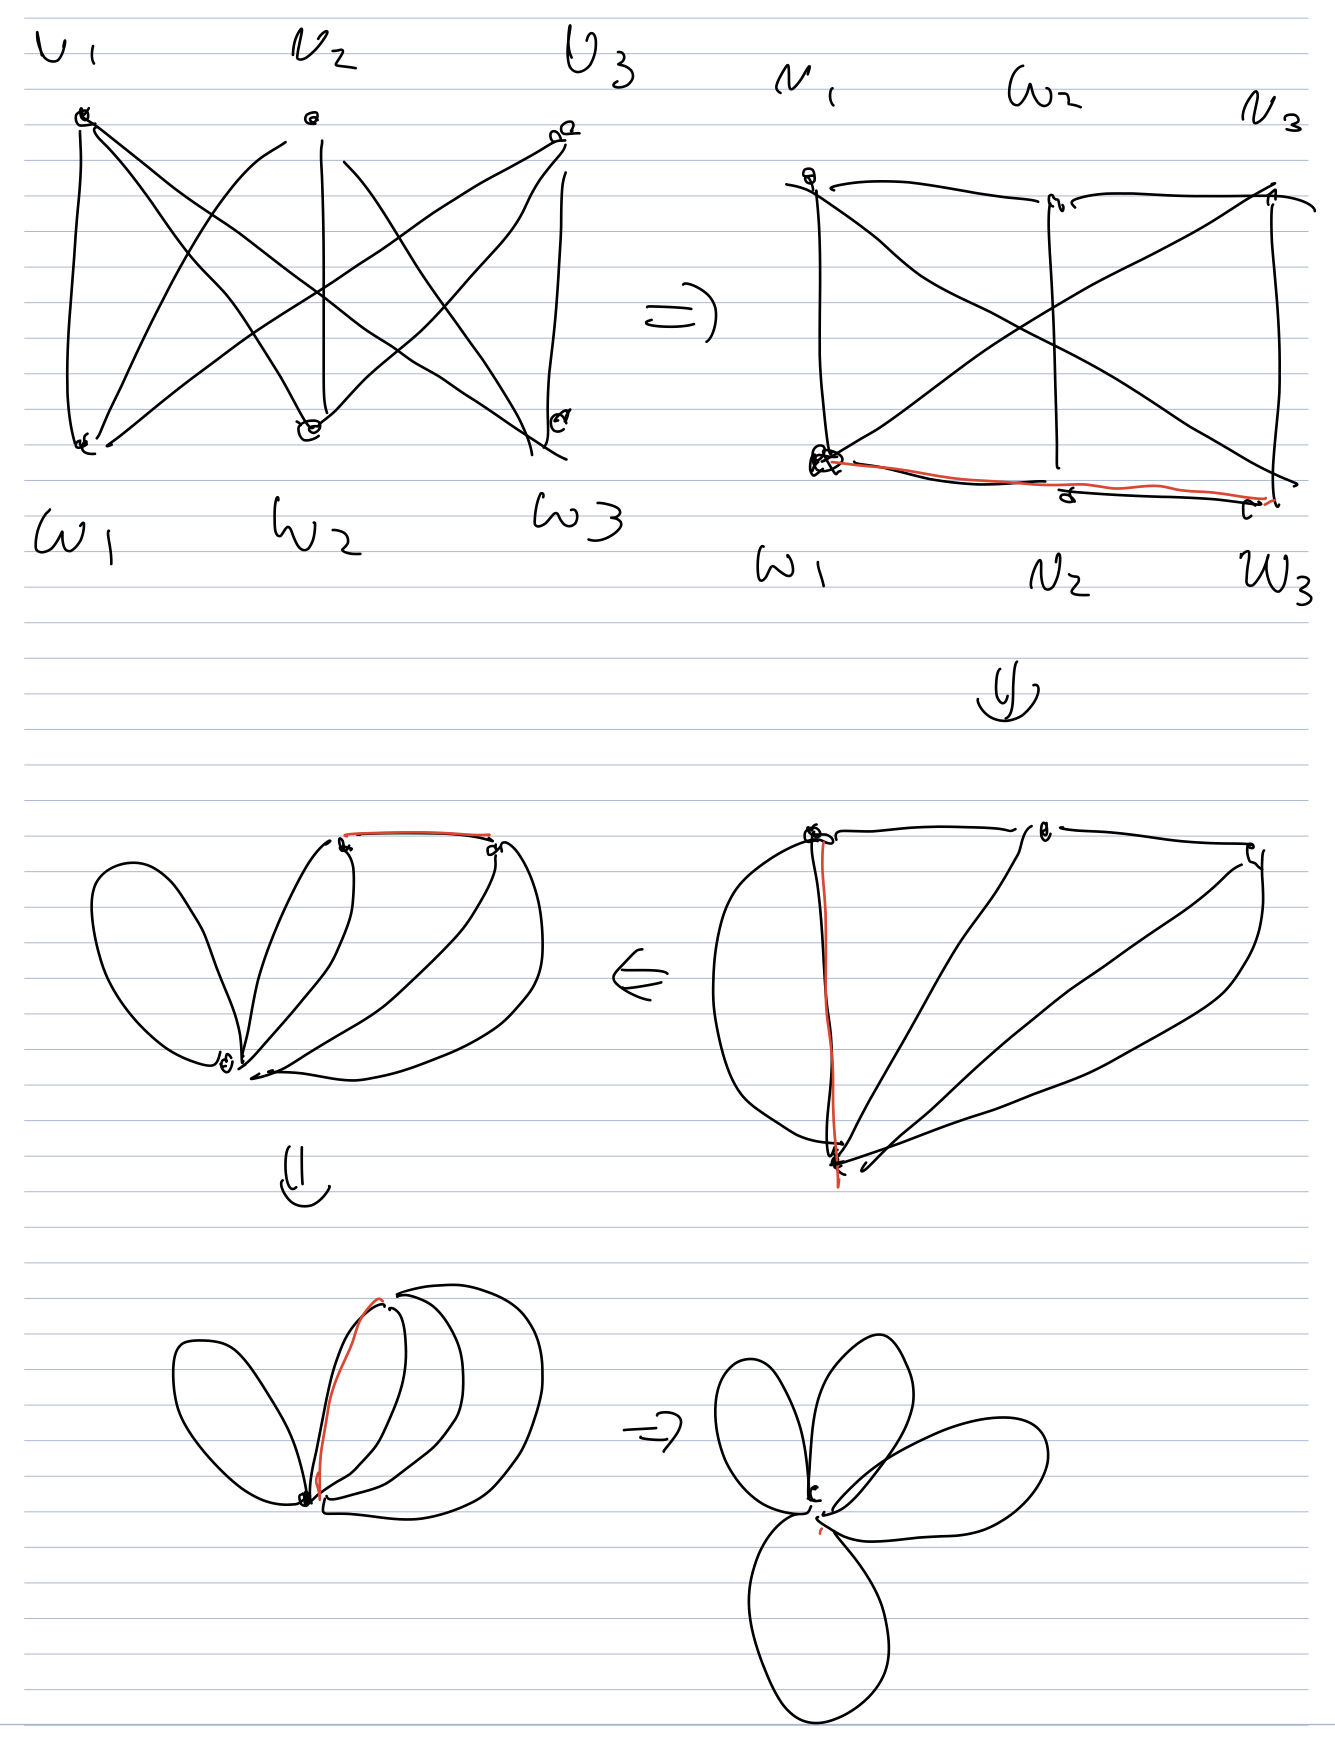
\includegraphics[width=.5\linewidth]{k33.jpeg}
   \caption{$K_{3, 3}$}
   \label{fig:k33}
 \end{figure}
 Figure \ref{fig:k33} shows that $K_{3, 3}$ is homotopy equivalent to $S^1 \vee S^1 \vee S^1 \vee S^1$.
 Thus the Van Kampen theorem implies that the fundamental group is the free group generated by 4 elements $\ev{ a, b, c, d }$ where each generator corresponds to each $S_1$.
\end{exer}

\begin{exer}{(Problem 2(b))}
  From Figure \ref{fig:k33}, it is clear that attaching four 2-cells, each killing one $S^1$, will give a simply connected space.
  We claim that 4 is the smallest number.

  When we attach 2-cells to the graph, the fundamental graph of the resulting space is $\ev{ a, b, c, d} / \ev{ r_1, r_2, \cdots }$ where each $r_i$ is the relation given by a product of $a, b, c, d$ in the order the boundary of the $i$th 2-cell was attached.
  Therefore, it suffices to show that $\ev{a, b, c, d} / \ev{r_1, r_2, r_3} \ne 0$.
  On the contrary, suppose that it is.
  
  If $\ev{a, b, c, d} / \ev{r_1, r_2, r_3} = 0$, then $\ev{a, b, c, d} = \ev{r_1, r_2, r_3}$.
  We will consider the surjective group homomorphism $\phi: \ev{a, b, c, d} \rightarrow \mathbb{Z}^4$ defined by $a \mapsto (1, 0, 0, 0), b \mapsto (0, 1, 0, 0), \cdots, d \mapsto (0, 0, 0, 1)$.
  Each $r_1, r_2, r_3$ is a product of $a, b, c, d$, so $\phi(r_i) = (d_{i, 1}, d_{i, 2}, d_{i, 3}, d_{i, 4})$ for some $d_{i, j} \in \mathbb{Z}$.
  Since $\ev{a, b, c, d} = \ev{r_1, r_2, r_3}$, $\phi(\ev{a, b, c, d}) = \phi(\ev{r_1, r_2, r_3})$.
  Since $\phi$ is surjective, $\phi(r_1), \phi(r_2), \phi(r_3)$ generate $\mathbb{Z}^4$.
  However, this implies $\{ \phi(r_1), \phi(r_2), \phi(r_3) \}$ is a basis of $\mathbb{R}^4$ because $\{ (1, 0, 0, 0), \cdots, (0, 0, 0, 1) \}$ is.
  This is clearly a contradiction, so we need at least four 2-cells.
\end{exer}

\begin{exer}{(Problem 3)}
  \begin{figure}[!htb]
    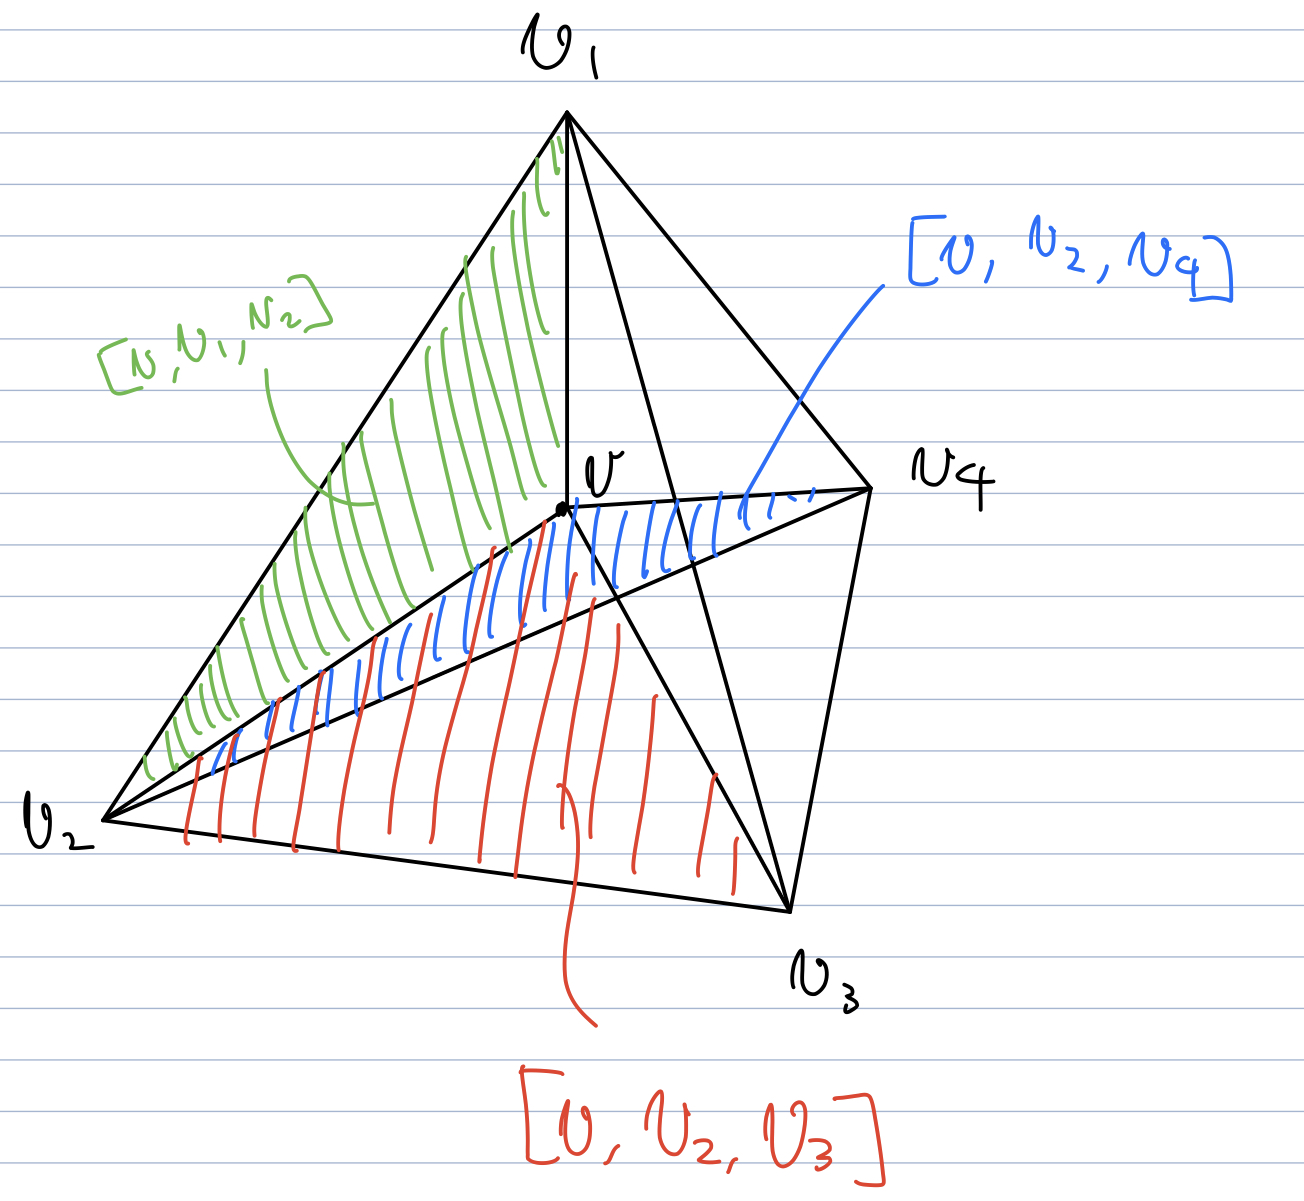
\includegraphics[width=.5\linewidth]{problem3.jpeg}
    \caption{Problem 3}
    \label{fig:problem3}
  \end{figure}
  Figure \ref{fig:problem3} shows what $X$ looks like.
  (It does not include all the faces in order to avoid cluttering the figure.)
  $X$ clearly deformation retracts to a point.
  Let $x \in X$.
  From Exercise 2.1.16(a) [a homework problem from Hatcher], the 0th homology groups are all 0 regardless of where $x$ is.

  For any $n \geq 1$, the exact sequence $\tilde{H}_n(X) \rightarrow \tilde{H}_n(X, X \setminus \{ x \}) \rightarrow \tilde{H}_{n - 1}(X \setminus \{ x \}) \rightarrow \tilde{H}_{n - 1}(X)$ shows that $\tilde{H}_n(X, X \setminus \{ x \}) \cong \tilde{H}_{n - 1}(X \setminus \{ x \})$ because $\tilde{H}_n(X) = \tilde{H}_{n - 1}(X) = 0$.
  We will calculate $\tilde{H}_n(X, X \setminus \{ x \}) = \tilde{H}_{n - 1}(X \setminus \{ x \})$ for each $n \geq 1$.
  There are five cases:
  \begin{enumerate}
    \item 
      Suppose $x = v_i$ for some $i$.
      Then $X \setminus \{ x \}$ deformation retracts to a point, so $\tilde{H}_n(X, X \setminus \{ x \}) = \tilde{H}_{n - 1}(X \setminus \{ x \}) = \tilde{H}_{n - 1}(\cdot) = 0$ for all $n \geq 1$.
    \item
      Suppose $x \in \Int([v_i, v_j])$ for some $i \ne j$.
      In other words, $x$ lies in the edge $v_iv_j$, and $x \ne v_i$ and $x \ne v_j$.
      This case is exactly the same as above because $X \setminus \{ x \}$ deformation retracts to a point,
    \item
      Suppose $x$ is on one of the faces.
      In other words, $v \in \Int([v, v_i, v_j])$ for some $i \ne j$.
      The space is homotopy equivalent to $S^1$, so $\tilde{H}_n(X, X \setminus \{ x \}) = \tilde{H}_{n - 1}(S^1)$.
      Therefore, $\tilde{H}_n(X, X \setminus \{ x \}) = \mathbb{Z}$ when $n = 2$ and 0 otherwise.
    \item
      Suppose $x = v$.
      Then the space is homotopy equivalent to the 1-skeleton of the 3-simplex.
      In other words, $X \setminus \{ x \}$ deformation retracts to a space consisting of 4 edges $[v, v_1], [v, v_2], [v, v_3], [v, v_4]$.
      Using a similar argument as Problem 2(a), we can see that it is homotopy equivalent to $S^1 \vee S^1 \vee S^1$.
      By Corollary 2.25, $\tilde{H}_n(X, X \setminus \{ x \}) = \mathbb{Z}^3$ when $n = 2$ and 0 otherwise.
    \item
      Suppose $x$ is on one of the edges from $v$.
      In other words, $x \in \Int([v, v_i])$ for some $i$.
      Without loss of generality, $i = 2$.
      Then the 3 faces shown in Figure \ref{fig:problem3} deformation retract to the edges $[v, v_i], [v_2, v_i]$ for each $i = 1, 3, 4$.
      Using a similar argument as Problem 2(a), we can see that it is homotopy equivalent to $S^1 \vee S^1$.
      By Corollary 2.25, $\tilde{H}_n(X, X \setminus \{ x \}) = \mathbb{Z}^2$ when $n = 2$ and 0 otherwise.
  \end{enumerate}
\end{exer}

\begin{exer}{(Problem 4)}
  As mentioned in Example 2.42 [Hatcher], $\RP^n$ has a CW structure with one cell $e^k$ in each dimensino $k \leq n$, and the attaching map for $e^k$ is the 2-sheeted covering projection $\phi: S^{k - 1} \rightarrow \RP^{k - 1}$.
  $X$ can be constructed by constructing $\RP^n$ as above and attaching an extra $e^n$ in the same manner that we attach the first $e^n$.
  Thus the cellular chain complex for $X$ is
  \begin{itemize}
    \item
      If $n$ is even, $0 \rightarrow \mathbb{Z}^2 \xrightarrow{\alpha} \mathbb{Z} \xrightarrow{0} \mathbb{Z} \xrightarrow{2} \mathbb{Z} \xrightarrow{0} \cdots \xrightarrow{2} \mathbb{Z} \xrightarrow{0} \mathbb{Z} \xrightarrow{2} \mathbb{Z} \xrightarrow{0} \mathbb{Z} \rightarrow 0$.
    \item
      If $n$ is odd, $0 \rightarrow \mathbb{Z}^2 \xrightarrow{\beta} \mathbb{Z} \xrightarrow{2} \mathbb{Z} \xrightarrow{0} \mathbb{Z} \xrightarrow{2} \cdots \xrightarrow{2} \mathbb{Z} \xrightarrow{0} \mathbb{Z} \xrightarrow{2} \mathbb{Z} \xrightarrow{0} \mathbb{Z} \rightarrow 0$.
  \end{itemize}
  It is clear that $d_k$ is the same as the one in the textbook for $k < n$.
  $\alpha$ is a map that sends $(a, b) \rightarrow 2a + 2b$ where each $a, b$ corresponds to each of the two $e^n$'s and each $a, b$ gets doubled for the same reason the $d_n$ in Example 2.42 is multiplication by 2.
  Similarly, $\beta$ is a map that sends $(a, b) \rightarrow 0$ where each $a, b$ gets sent to 0 and 0 + 0 = 0.
  From this, it follows that

  \begin{align*}
    H_{n}(X) = \begin{cases}
      \mathbb{Z}^2 & \text{for $k = n =$ odd,} \\
      \mathbb{Z} & \text{for $k = n =$ even or $k = 0$,} \\
      \mathbb{Z}_2 & \text{for $k$ odd, $0 < k < n$,} \\
      0 & \text{otherwise.} \\
    \end{cases}
  \end{align*}
\end{exer}

\begin{exer}{(Problem 5(a))}
  Let $X = S^1 \times S^2$ and $Y = S^1 \vee S^2 \vee S^3$.
  \begin{align*}
    \pi_1(S^1 \times S^2)
      &= \pi_1(S^1) \times \pi_1(S^2) & \text{(Proposition 1.12)} \\
      &= \mathbb{Z} \times 0 \\
      &= \mathbb{Z}. \\
    \pi_1(S^1 \vee S^2 \vee S^3)
      &= \pi_1(S^1) * \pi_1(S^2) * \pi_1(S^3) & \text{(Van Kampen)} \\
      &= \mathbb{Z} * 0 * 0 \\
      &= \mathbb{Z}.
  \end{align*}

  $X$ and $Y$ are both path connected, so $H_0(X) = H_0(Y) = \mathbb{Z}$.

  We will consider two subspaces of $X$ the union of whose interiors equals $X$.
  Identify each point of $X = S^1 \times S^2$ by a pair of coordinates $(\theta, (x, y, z))$ where $\theta$ is the angle in $S^1$ and $(x, y, z)$ satisfies $x^2 + y^2 + z^2 = 1$.
  Let $A = \{ (\theta, (x, y, z)) \mid -\epsilon \leq \theta \leq \pi + \epsilon \}, B = \{ (\theta, (x, y, z)) \mid \pi - \epsilon \leq \theta \leq 2\pi + \epsilon \}$ where $\epsilon > 0$ is a small number.
  Then each $A$ and $B$ deformation retracts to a space homeomorphic to $S^2$.
  $A \cap B$ consists of two path components, each of which deformation retracts to a space homeomorphic to $S^2$.
  The homology groups of $A \cap B$ are relatively easy to calculate because $H_n(A \cap B) = H_n(S^2 \coprod S^2) = H_n(S^2) \oplus H_n(S^2)$ by Proposition 2.6 for any $n$.
  Moreover, it is clear that $\Int(A) \cup \Int(B) = X$.
  We will consider the Mayer-Vietoris sequence formed by $A, B \subset X$.

  First, we will consider the sequence $H_n(A) \oplus H_n(B) \rightarrow H_n(X) \rightarrow H_{n - 1}(A \cap B)$ for each $n \geq 4$.
  $H_n(A) = H_n(B) = H_{n - 1}(A \cap B) = 0$ for $n \geq 4$
  By the exactness, $H_n(X) = 0$ for all $n \geq 4$.
  Next, we will consider the following sequence:

  \begin{align*}
    &\tilde{H}_3(A \cap B) \rightarrow \tilde{H}_3(A) \oplus \tilde{H}_3(B) \rightarrow \tilde{H}_3(X) \xrightarrow{\alpha} \\
    &\tilde{H}_2(A \cap B) \xrightarrow{\beta} \tilde{H}_2(A) \oplus \tilde{H}_2(B) \xrightarrow{\gamma} \tilde{H}_2(X) \rightarrow \\
    &\tilde{H}_1(A \cap B) \rightarrow \tilde{H}_1(A) \oplus \tilde{H}_1(B) \rightarrow \tilde{H}_1(X) \rightarrow \\
    &\tilde{H}_0(A \cap B) \rightarrow \tilde{H}_0(A) \oplus \tilde{H}_0(B).
  \end{align*}

  $\tilde{H}_3(A \cap B) = \tilde{H}_3(A) = \tilde{H}_3(B) = \tilde{H}_1(A \cap B) = \tilde{H}_1(A) = \tilde{H}_1 = \tilde{H}_0(A) = \tilde{H}_0(B) = 0$, and $\tilde{H}_0(A \cap B)$.
  By replacing the exact sequence with those values and splitting the sequence into two for readability, we obtain the following sequences:
  \begin{gather*}
    0 \rightarrow \tilde{H}_3(X) \xrightarrow{\alpha} \tilde{H}_2(A \cap B) \xrightarrow{\beta} \tilde{H}_2(A) \oplus \tilde{H}_2(B) \xrightarrow{\gamma} \tilde{H}_2(X) \rightarrow 0, \\
    0 \rightarrow \tilde{H}_1(X) \rightarrow \mathbb{Z} \rightarrow 0.
  \end{gather*}

  By the exactness, we can conclude that $\tilde{H}_1(X) \cong \mathbb{Z}$.
  We will examine the homomorphism $\beta$ to understand the sequence.
  $\tilde{H}_2(A \cap B) = \ev{[a], [b] \mid [[a], [b]]}$ where each $a, b$ lives in $A \cap B$ and $a$ lives in one of the path components of $A \cap B$ and $b$ lives in the other.
  Moreover, $[a] = [b]$ in $\tilde{H}_2(A)$ and $\tilde{H}_2(B)$.
  (Based on orientation, $[a] = -[b]$, but we can simply change the orientation of $[b]$ in that case.)
  Then $\beta(c_1[a] + c_2[b]) = ((c_1 + c_2)[a], (c_1 + c_2)[a])$.
  This gives us that $\Im(\alpha) = \ker(\beta) = \{ c[a] - c[b] \mid c \in \mathbb{Z} \} = \mathbb{Z}$.
  By the exactness, $\alpha$ is injective, so $\tilde{H}_3(X) = \mathbb{Z}$.
  Moreover, $\ker(\gamma) = \Im(\beta) = \{ (c[a], c[a]) \mid c \in \mathbb{Z} \}$.
  By the exactness, $\gamma$ is surjective, so $\tilde{H}_2(X) = (\tilde{H}_2(A) \oplus \tilde{H}_2(B)) / \Im(\beta) = \ev{[a]} \oplus \ev{[a]} / \ev{([a], [a])} = \mathbb{Z}$.
  Since reduced homology groups and homology groups are identical when $n \geq 2$, we have
  \begin{align*}
    H_n(X) &= \begin{cases}
      \mathbb{Z} & (n = 0, 1, 2, 3) \\
      0 & (n \geq 4).
    \end{cases}
  \end{align*}


  By Corollary 2.25, $\tilde{H}_n(S^1 \vee S^2 \vee S^3) = \tilde{H}_n(S^1) \otimes \tilde{H}_n(S^2) \otimes \tilde{H}_n(S^3)$.

  Therefore,
  \begin{align*}
    \tilde{H}_n(Y) = \begin{cases}
      \mathbb{Z} & (n = 1, 2, 3) \\
      0 & (n = 0, n \geq 4).
    \end{cases}
  \end{align*}

  For $n \geq 1$, $\tilde{H}_n(Y) = H_n(Y)$, so $H_0(Y) = H_1(Y) = H_2(Y) = H_3(Y) = \mathbb{Z}$ and $H_n(Y) = 0$ for all $n \geq 4$.
\end{exer}

\begin{exer}{(Problem 5(b))}
  We claim that the universal cover is $\mathbb{R} \times S^2$.
  $p(\theta, (x, y, z)) = ((\cos \theta, \sin \theta), (x, y, z))$ is a covering map.
  Moreover, $\pi_1(\mathbb{R} \times S^2) = \pi_1(\mathbb{R}) \times \pi_1(S^2) = 0 \times 0 = 0$, so $\mathbb{R} \times S^2$ is simply connected.
  Therefore, $\mathbb{R} \times S^2$ is indeed a universal cover of $X$.

  $\mathbb{R} \times S^2$ is homeomorphic to $(0, 1) \times S^2$.
  This space deformation retracts to $S^2$ because $(0, 1) \times S^2$ is homeomorphic to an open ball with its center removed.
  Thus their homology groups are $H_2(\tilde{X}) = H_0(\tilde{X}) = \mathbb{Z}$ and $H_n(\tilde{X}) = 0$ for all other $n$.
\end{exer}

\begin{exer}{(Problem 5(c))}
  \begin{figure}[!htb]
    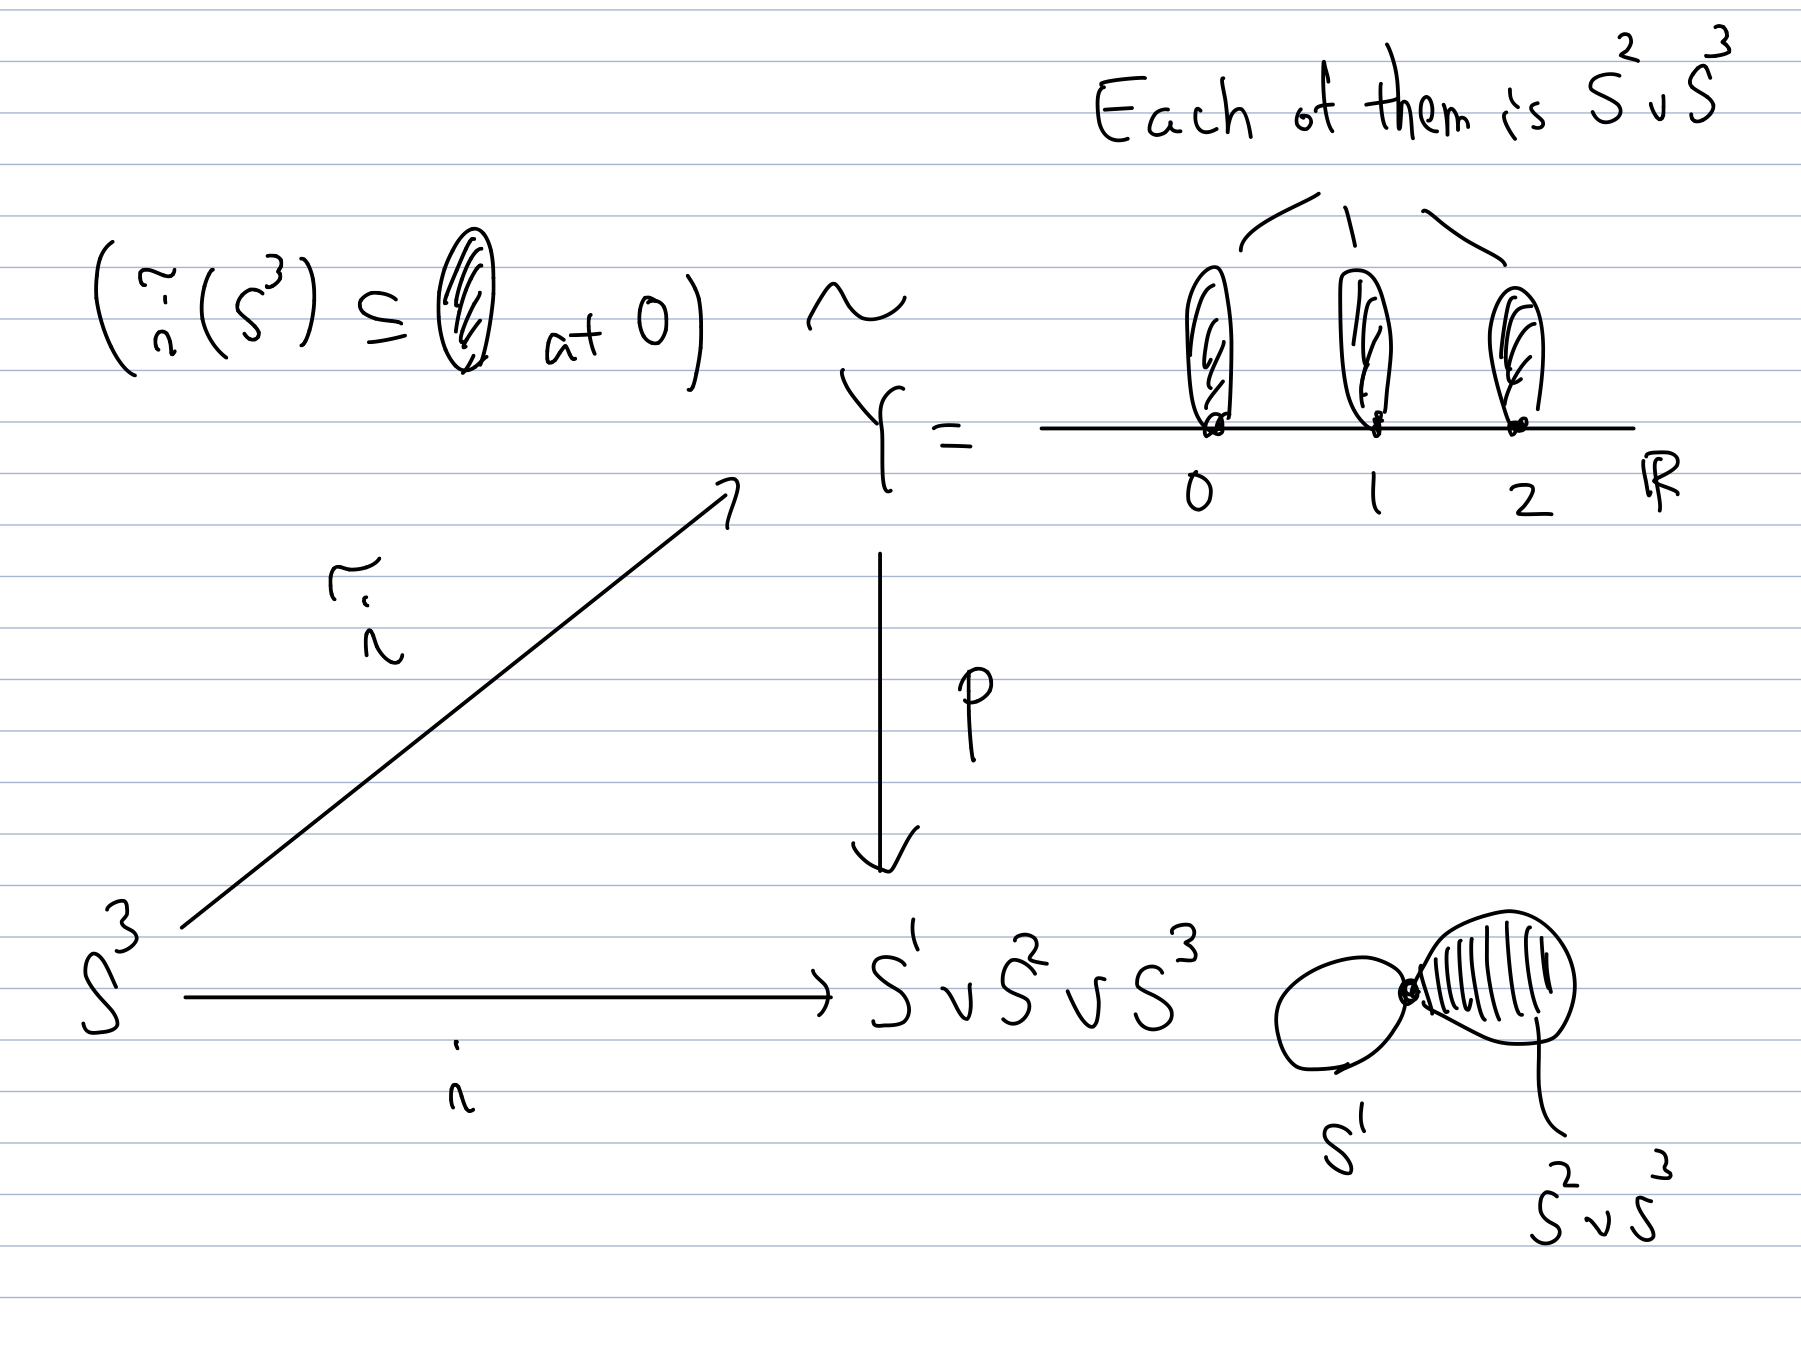
\includegraphics[width=.8\linewidth]{problem5_c.jpeg}
    \caption{Problem 5(c)}
    \label{fig:5c}
  \end{figure}
  We claim that the universal covering space is the real line with $S^2 \vee S^3$ attached to each of its integral points (Figure \ref{fig:5c}).
  Since $S^2$ and $S^3$ are both contractible, the wedge sum must be contractible.
  Attaching contractible spaces to each integral point of $\mathbb{R}$, which itself is contractible, gives a contractible space.
  The covering map $p$ can be defined in an obvious way.
  Every point on $\mathbb{R}$ can be mapped to $S^1$ by $\theta \rightarrow (\cos(\theta), \sin(\theta))$, and each copy of $S^2 \vee S^3$ can be mapped identically to $S^2 \vee S^3$.
  The $i$ in Figure \ref{fig:5c} is the obvious inclusion map, and $\tilde{i}$ sends $S^3$ into the copy of $S^2 \vee S^3$ that is attached to 0 on $\mathbb{R}$.
  (It does not matter which copy, but it is necessary to specify which.)
  Then the diagram clearly commutes.

  By the Mayer-Vietoris sequence, we have an exact sequence $H_3((S^1 \vee S^2) \cap S^3) \rightarrow H_3(S^1 \vee S^2) \oplus H_3(S^3) \xrightarrow{\psi} H_3(S^1 \vee S^2 \vee S^3) \rightarrow H_2((S^1 \vee S^2) \cap S^3)$.
  (To be precise, we need $S^1 \vee S^2$ with a small neighborhood and $S^3$ with a small neighborhood, such that the union of the interiors is $S^1 \vee S^2 \vee S^3$ and the intersection deformation retracts onto a point.)
  Then $H_n((S^1 \vee S^2) \cap S^3) = 0$ for $n = 2, 3$.
  Therefore, $\psi$ is an isomorphism.
  $H_3(S^1 \vee S^2) = 0$ by the Mayer-Vietoris sequence $0 = H_3(S^1) \oplus H_3(S^2) \rightarrow H_3(S^1 \vee S^2) \rightarrow H_3(S^1 \cap S^2) = 0$ where $S^1, S^2 \subset S^1 \vee S^2$ are technically $S^1$ and $S^2$ with a small neighborhood.
  Therefore, instead of $\psi$, we can consider the map $\psi': H_3(S^3) \rightarrow H_3(S^1 \vee S^2 \vee S^3)$ defined by $\psi'(x) = \psi(0, x)$.
  By construction of the Mayer-Vietoris sequence, $\psi'$ is induced by the inclusion map $i$.
  Since homology is a covariant functor, $p^{*}$ and $\tilde{i}^{*}$, which are induced by $p$ and $\tilde{i}$, must commute with $\psi' = i^{*}$.
  In other words, $i^{*} = \psi' = p^{*} \circ \tilde{i}^{*}$.
  Since $i^{*}$ is an isomorphism, $\tilde{i}^{*}$ must be injective.
  This implies $H_3(\tilde{Y})$ contains an isomorphic copy of $H_3(S^3) = \mathbb{Z}$.

  We calculate in Part (b) that $H_3(\tilde{X}) = 0$.
  Therefore, $H_3(\tilde{X}) \ne H_3(\tilde{Y})$.
\end{exer}

\begin{exer}{(Problem 6)}
  By Proposition 1.32, Theorem 1.38 and Proposition 1.39, it suffices to find a subgroup of $\pi_1(\Sigma_g)$ whose index is 3 and check whether it is normal.

  Let $g = 0$.
  Then $\pi_1(\Sigma_g) = 0$.
  There does not exist an index-3 subgroup.
  Therefore, there exists no non-normal, connected, 3-sheeted cover.

  Let $g = 1$.
  Then $\Sigma_g$ is a torus, so the fundamental group of $\Sigma_g$ is $\ev{ a, b \mid [a, b] }$.
  Since it is abelian, all the subgroups are normal.
  Therefore, there exists no non-normal, connected, 3-sheeted cover.

  Let $g \geq 2$.
  Then $\pi_1(\Sigma_g) = \ev{a_1, b_1, a_2, b_2, \cdots, a_g, b_g \mid [a_1, b_1] \cdots [a_g, b_g]}$.
  Consider the homomorphism $\phi: \pi_1(\Sigma_g) \rightarrow S_3$ such that
  \begin{itemize}
    \item
      $a_1 \mapsto (123)$.
    \item
      $a_2 \mapsto (12)$.
    \item
      $a_i \mapsto (1)$ for all $i \geq 3$ and $b_i \mapsto (1)$ for all $i$.
  \end{itemize}
  This is indeed a homomorphism because 
  \begin{align*}
    \phi([a_1, b_1] \cdots [a_g, b_g])
        &= \phi([a_1, b_1])\phi([a_2, b_2]) \\
        &= (123)(123)^{-1}(12)(12)^{-1} \\
        &= (1).
  \end{align*}
  Moreover, $\phi$ is surjective.
  Let $H$ be the subgroup generated by $a_1^3, a_2, \cdots, a_g, b_1, \cdots, b_g$.
  Thus $H$ is an index-3 subgroup of $\pi_1(\Sigma_g)$.
  Then there are three distinct cosets, $H, a_1H, a_1^2H$.
  $\phi(H) = \ev{(12)}$ because $\phi(a_1^3) = (123)^3 = (1)$.
  Suppose $H$ is normal.
  Then $a_1b_1a_1^{-1} \in H$.
  This implies $\phi(a_1b_1a_1^{-1}) \in \phi(H) = \ev{(12)}$, but $\phi(a_1)\phi(b_1)\phi(a_1)^{-1} = (123)(12)(132) = (23) \notin \ev{(12)}$.
  This is a contradiction, so $H$ cannot be normal.
  We found a non-normal index-3 subgroup of $\pi_1(\Sigma_g)$, so there exists a non-normal, connected, 3-sheeted cover.
\end{exer}

\end{document}


